\chapter{Результаты}
\label{chap:results}
\section{Производительность}
Ввиду большой связности компонентов нейронной сети между собой линейный рост количества нейронов выливается в квадратичный рост сложности вычислений, так как число соединений между нейронами при достаточно малом количестве нейронов растет в квадрате от их числа (до того момента, как число нейронов превысит 4000 штук)
Для измерения потребления ресурсов компьютера в ходе экспериментов полученный программный код был запущен несколько раз, с различным количеством нейронов в общей сложности.

Как видно на рисунке \ref{fig:perf_syn}, отчетливо прослеживается нелинейная взаимосвязь между количеством нейронов и синапсов. График выглядит как квадратичная функция.

\begin{figure}
	\centering
	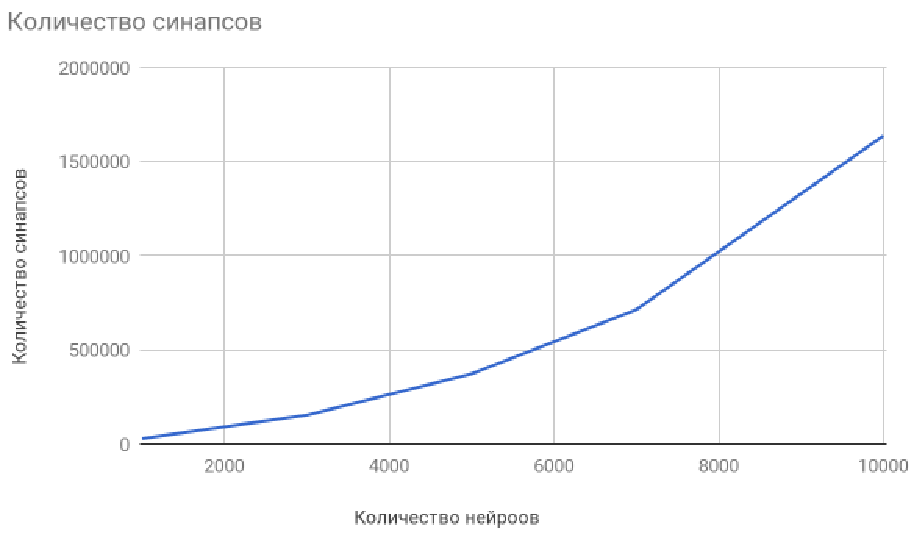
\includegraphics[width=\linewidth]{perf_syn}
	\caption{Количество синапсов.}
	\label{fig:perf_syn}
\end{figure}

На рисунке \ref{fig:perf_time}, изображена зависимость скорости исполнения от количества нейронов, данный график так же представляет собой квадратичную функцию, что интуитивно понятно, учитывая что график роста количества синапсов имеет прямое влияние на скорость вычислений, что в свою очередь выдает результат, растущий подобным скорости роста количества вычислений образом.

\begin{figure}
	\centering
	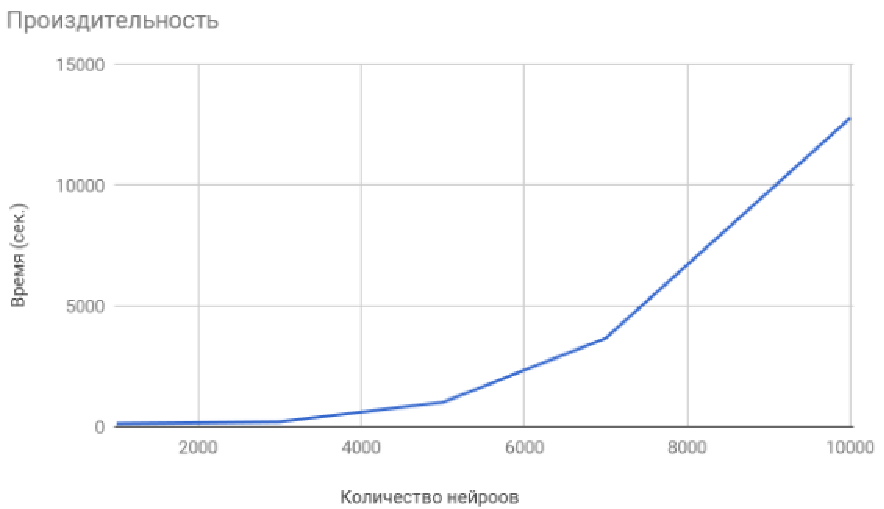
\includegraphics[width=\linewidth]{perf_time}
	\caption{Время исполнения.}
	\label{fig:perf_time}
\end{figure}

Однако, потребление памяти на рисунке \ref{fig:perf_mem} имеет слегка отличный график роста. Данное явление объяснимо необходимостью дополнительных аллокаций для ядра симуляции \en{NEST} и сборкой мусора в \en{Python}. Несмотря на это, график имеет нелинейный порядок роста.
\begin{figure}
	\centering
	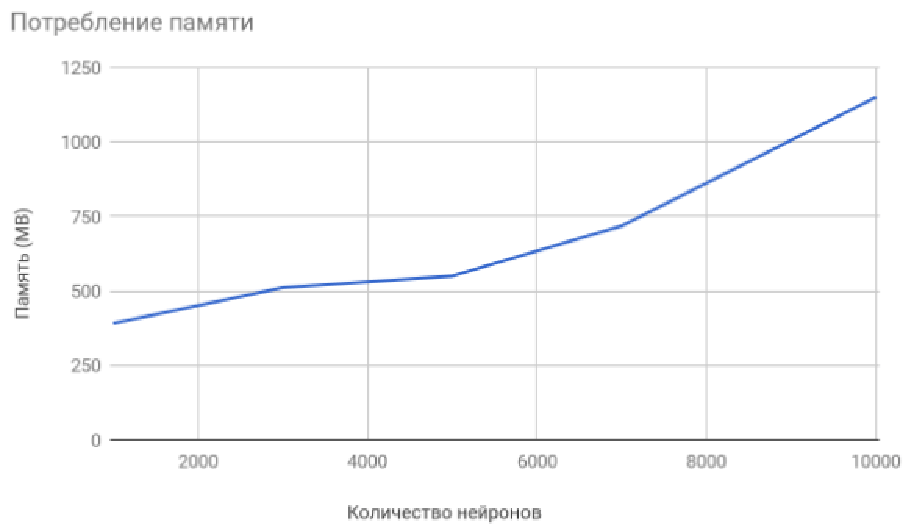
\includegraphics[width=\linewidth]{perf_mem}
	\caption{Потребление памяти.}
	\label{fig:perf_mem}
\end{figure}


\section{Результаты эксперимента}
\section{Стимуляция моторной коры с эмоциональной мотивацией}
На изображении \ref{fig:exp_motor} представлена активность моторной коры во время симуляции. 
Симулируется эмоциональная оценка в течении отрезка времени с 100 мс. до 450 мс., после чего включается генерация потенциалов действия на моторной коре (400, 550), полученная в результате моторная активность, подкрепленная эмоциональным стимулом получается гораздо значительней, нежели симуляция какого-нибудь компонента в отдельности. В отрезок времени с 700-800 мс. работает лишь стимулирование спайковой активности в моторной коре.

\begin{figure}
	\centering
	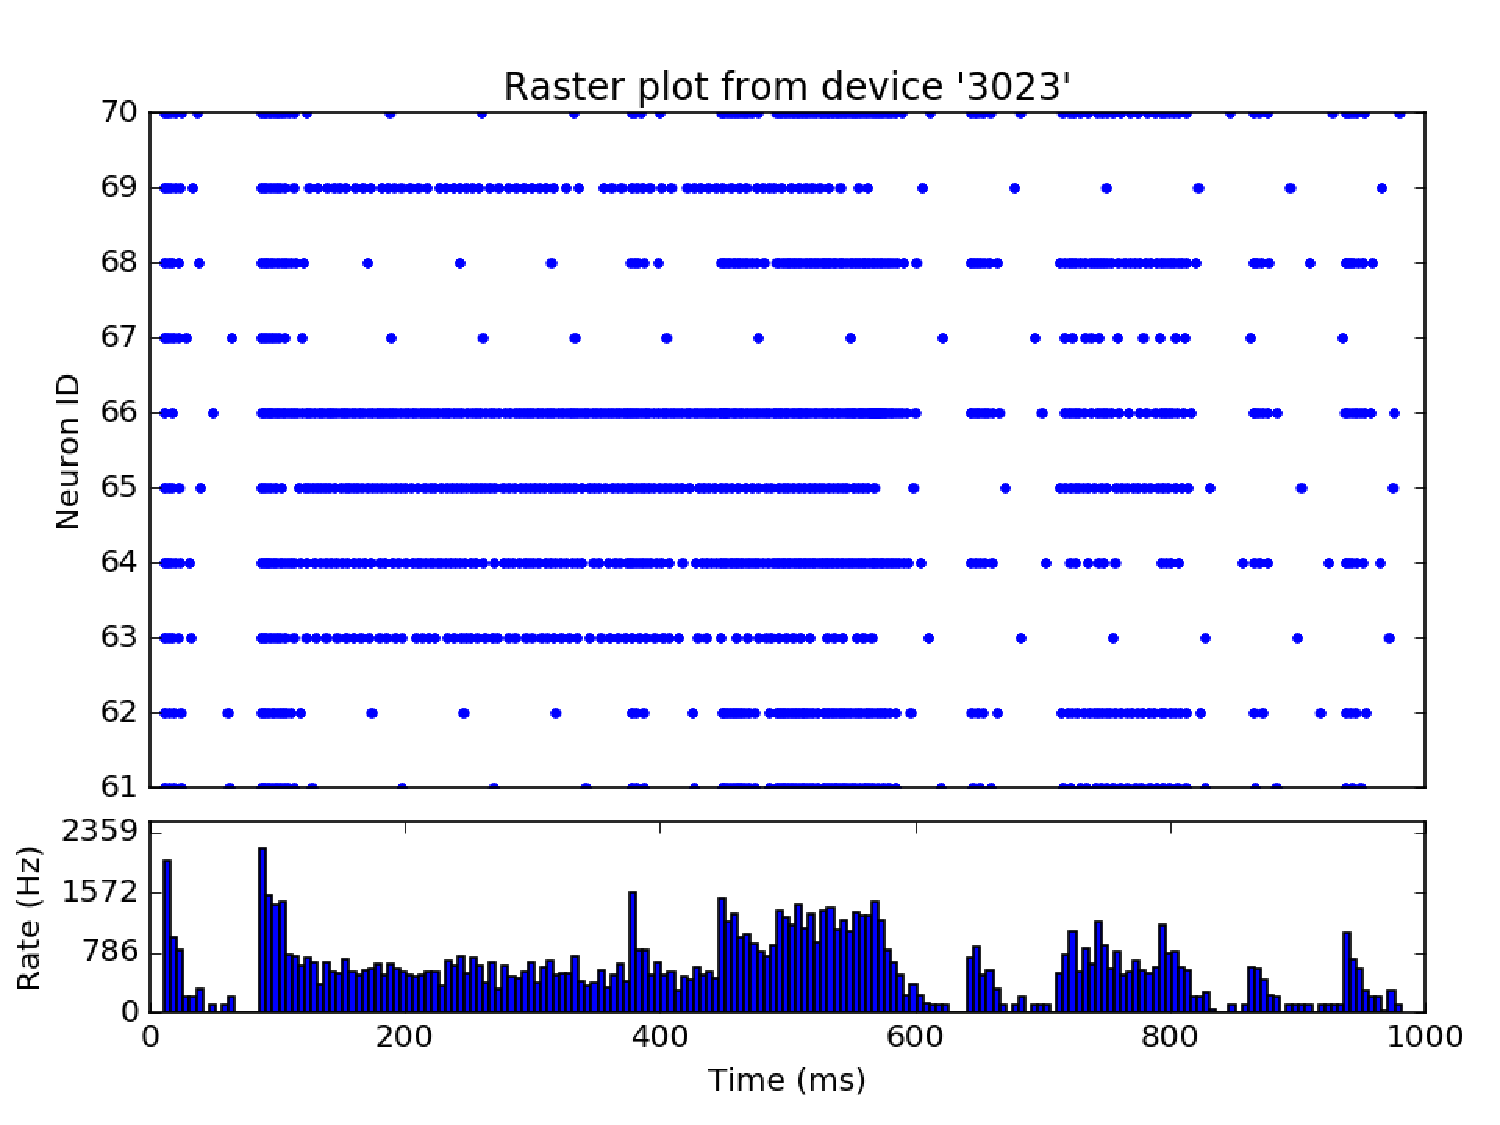
\includegraphics[width=\linewidth]{exp_motor}
	\caption{Нейрональная активность в моторной коре в течении симуляции.}
	\label{fig:exp_motor}
\end{figure}

\section{Влияние афферентных путей на систему}
Эксперимент составлен согласно плану \ref{section:validation2}.
Запускается симулирование эмоции \enquote{удивление}, после чего, ближе к ее концу запускается сигнал вверх по восходящему спиноталамического пути информация о неожиданном интенсивном взаимодействии со средой, в результате данного эксперимента активность на спинном мозге резко возрастает, что в свою очередь вызывает дополнительную активность в мышцах.
Влияние данного стимулирования хорошо прослеживается сквозь весь нисходящий кортикоспинальный тракт.

На рис. \ref{fig:exp2_cells} изображена активность нейронов на самом нижнем уровне восходящего спиноталамического тракта.
Это имеет следующие последствия для нисходящего тракта на уровне спинного мозга: рис \ref{fig:exp2_spine}. На изображении виден резкий подъем активности спинного мозга, а затем, его медленный спад, в связи с отключением стимуляции эмоциональной системы. И, его полное угасание из-за отключения генератора спайков на восходящем тракте.

\begin{figure}
	\centering
	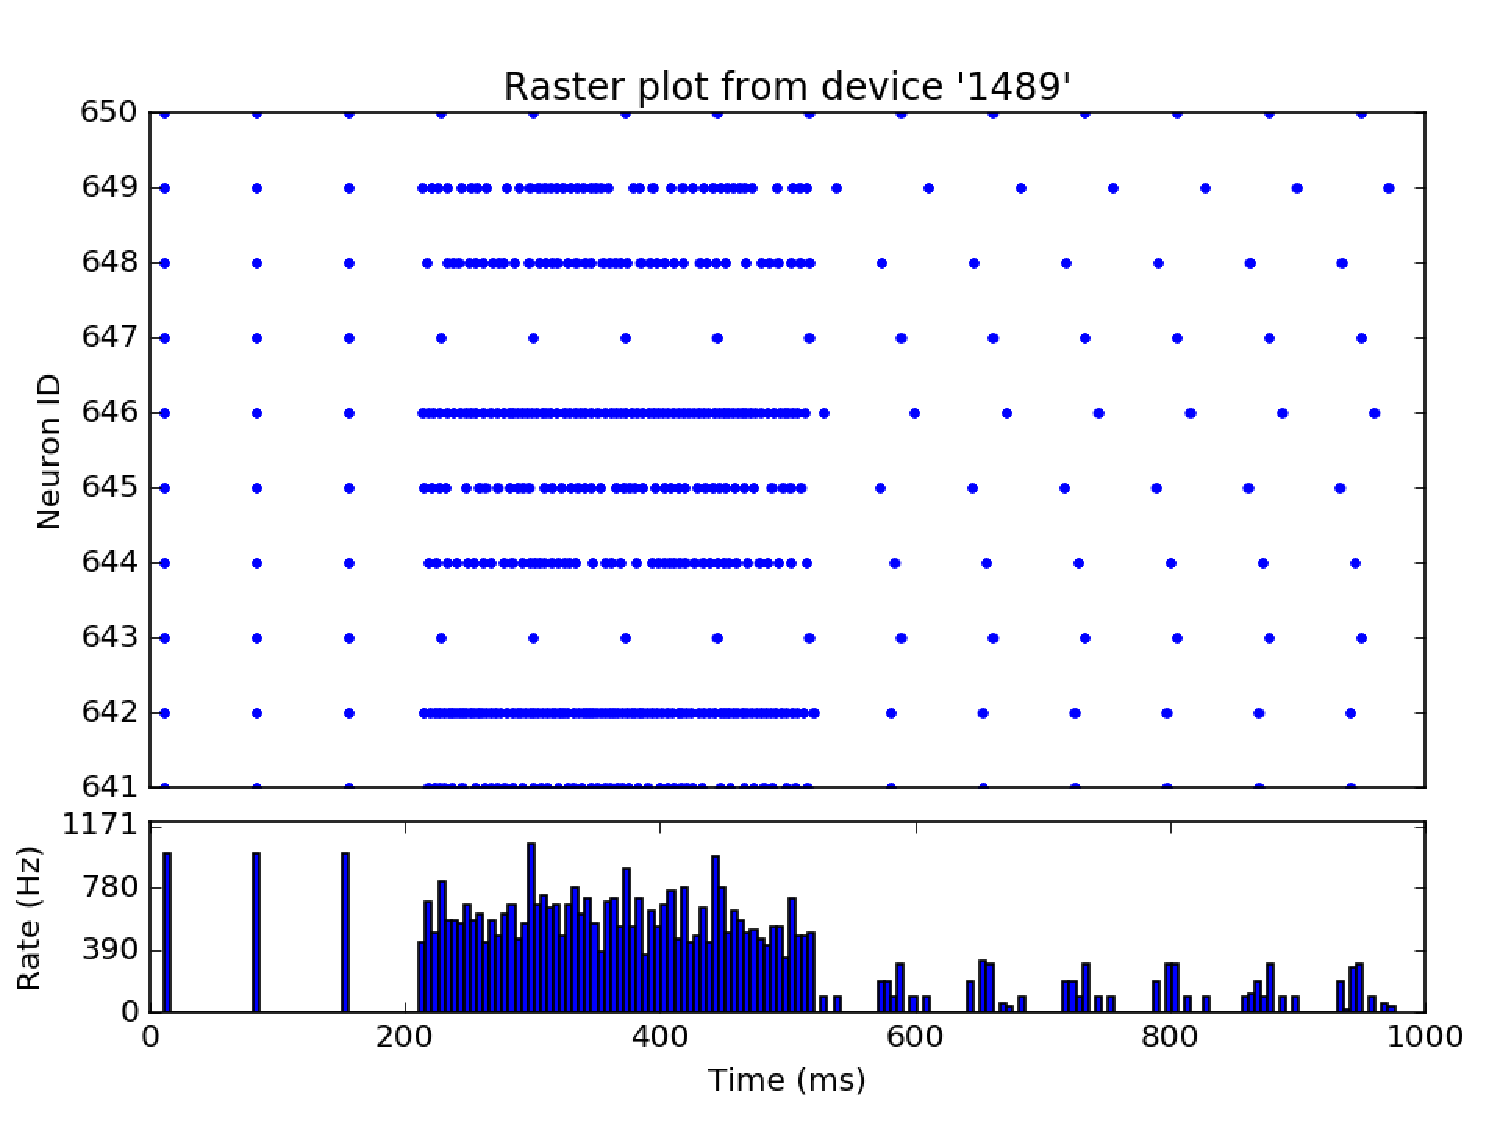
\includegraphics[width=\linewidth]{exp2_cells}
	\caption{Нейронная активность в чувствительных клетках тела.}
	\label{fig:exp2_cells}
\end{figure}
\begin{figure}
	\centering
	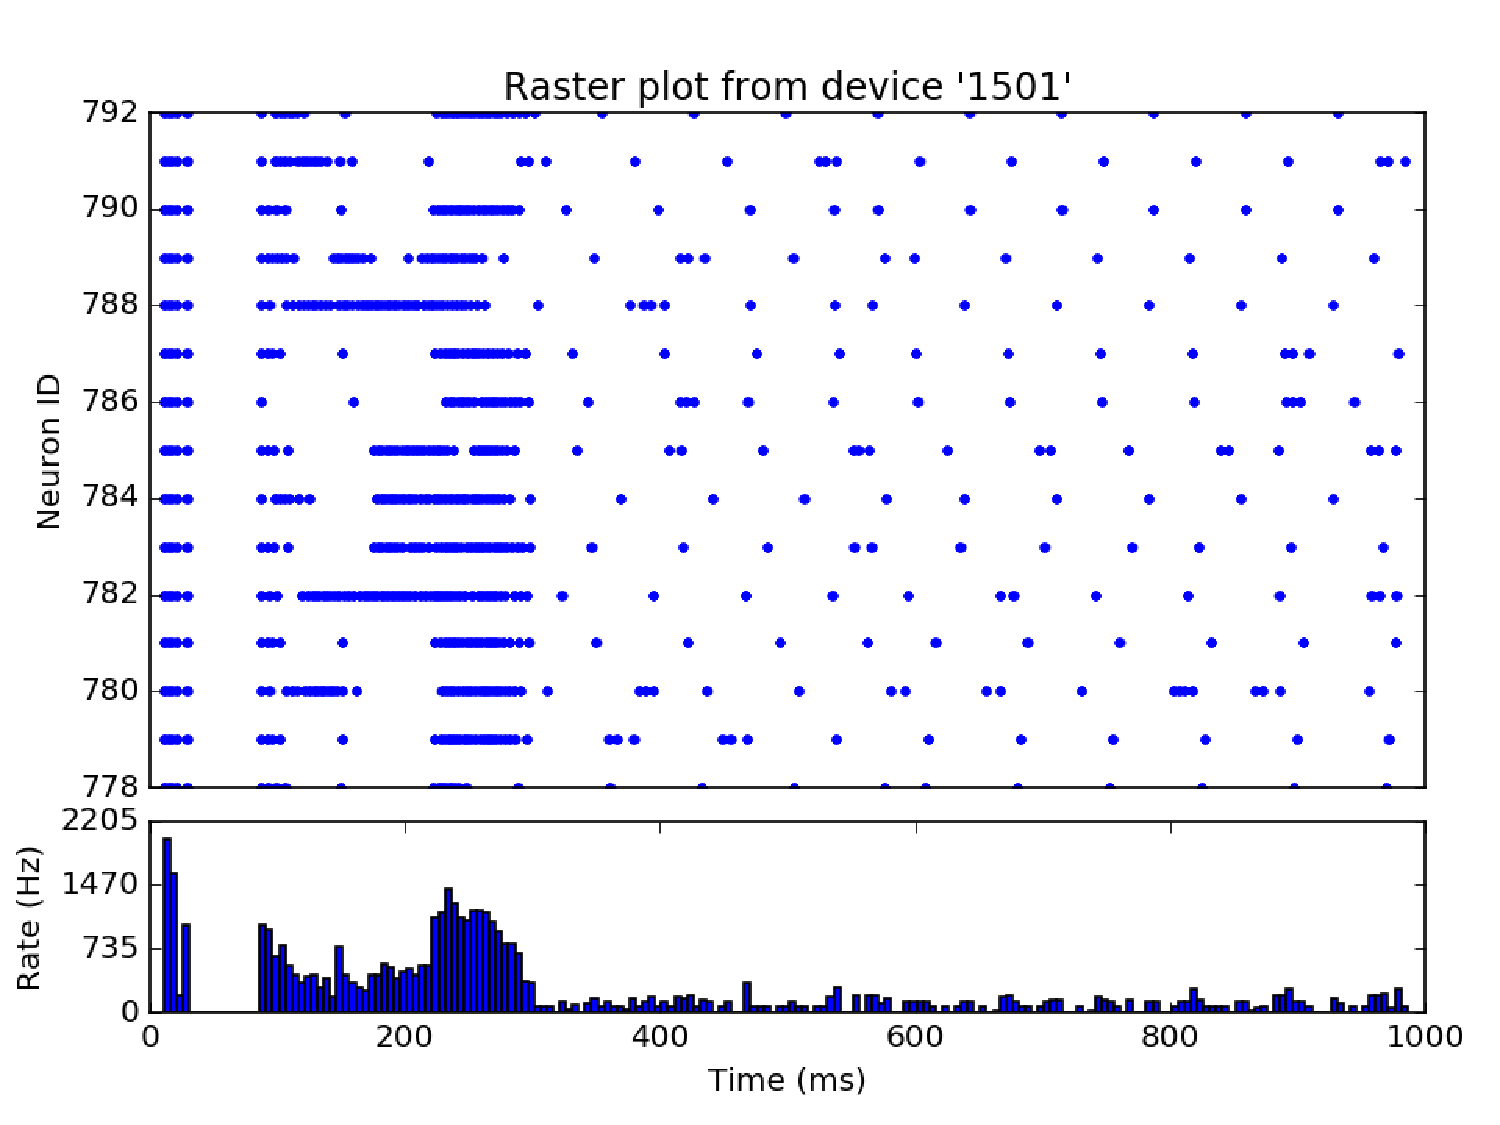
\includegraphics[width=\linewidth]{exp2_spine}
	\caption{Нейронная активность в спинном мозгу.}
	\label{fig:exp2_spine}
\end{figure}